They differ since they now need to recalculate the angle error when the
angle error gets to large. In Figure~\ref{fig:task17} we can see that
$d_p$ increses when the robot starts translation, it will then need to
correct itself on the move.

\begin{figure}[H]
    \centering
    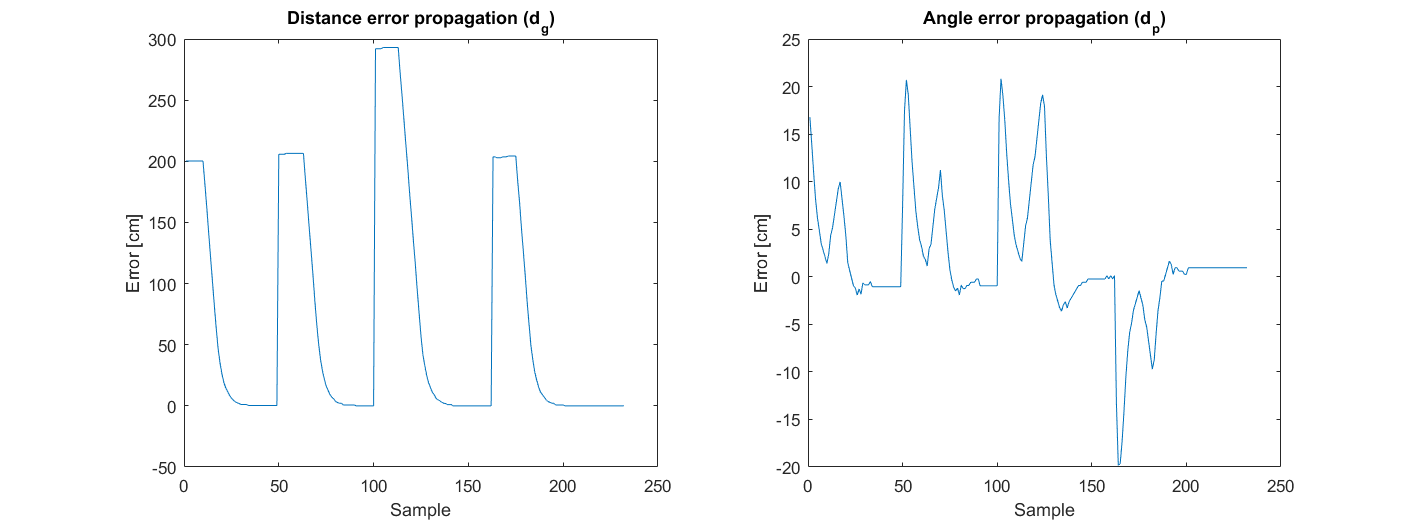
\includegraphics[width=\textwidth]{../matlab/images/task17.png}
    \caption{Control performance when both controllers is activated}
    \label{fig:task17}
\end{figure}
